\documentclass[12pt,a4paper]{report}

% Packages
\usepackage[utf8]{inputenc}
\usepackage{geometry}
\geometry{a4paper, margin=1in}
\usepackage{graphicx}
\usepackage{hyperref}
\usepackage{titlesec}
\usepackage{setspace}
\usepackage{listings}
\usepackage{xcolor}
\usepackage{tocbibind}
\usepackage{float}
\usepackage{enumitem}
\usepackage{booktabs}
\usepackage{tikz}
\usepackage{pdflscape}
\usepackage{tabularx}
\usepackage{longtable}
\usepackage{rotating}
\usepackage[space]{grffile}
\graphicspath{{src/image/}{src/Information artitecture/}}

% Code Listing Style
\definecolor{codegreen}{rgb}{0,0.6,0}
\definecolor{codegray}{rgb}{0.5,0.5,0.5}
\definecolor{codepurple}{rgb}{0.58,0,0.82}
\definecolor{backcolour}{rgb}{0.95,0.95,0.92}

\lstdefinestyle{mystyle}{
    backgroundcolor=\color{backcolour},   
    commentstyle=\color{codegreen},
    keywordstyle=\color{magenta},
    numberstyle=\tiny\color{codegray},
    stringstyle=\color{codepurple},
    basicstyle=\ttfamily\footnotesize,
    breakatwhitespace=false,         
    breaklines=true,                 
    captionpos=b,                    
    keepspaces=true,                 
    numbers=left,                    
    numbersep=5pt,                  
    showspaces=false,                
    showstringspaces=false,
    showtabs=false,                  
    tabsize=2
}
\lstset{style=mystyle}

% Title Page Information
\title{
    \vspace{2cm}
    \Huge \textbf{GeoMNREGA Portal}\\
    \Large A Modern React-Based Geospatial Research Dashboard\\
    \vspace{1cm}
    \large Project Report
}
\author{
    \textbf{Deepak Meena} \\ \textit{Lead Portal Developer} \\
    \and
    \textbf{Pradeep Singh} \\ \textit{Data Engineering \& Consolidation}
}
\date{
    \vspace{1cm}
    \textbf{Under the Guidance of:} \\
    \textbf{Gaurav Arora} \\ \textit{Advisor} \\
    \textbf{Saif Ali} \\ \textit{Co-Advisor} \\
    \vspace{1cm}
    \today
}

\begin{document}
\begin{spacing}{1.5}

% Title Page
\maketitle
\thispagestyle{empty}

\begin{center}
    \textbf{GitHub Repository:} \url{https://github.com/deepakm0003/GeoMnrega-Portal-Lab}
\end{center}

\newpage

% Abstract
\chapter*{Abstract}
\addcontentsline{toc}{chapter}{Abstract}
The GeoMNREGA Portal is an advanced academic research visualization platform designed to explore and analyze geospatial datasets related to the Mahatma Gandhi National Rural Employment Guarantee Act (MNREGA) and Water Infrastructure (MICES) across Indian states and districts. This project leverages modern web technologies including React 18, Vite, Mapbox GL JS, and Tailwind CSS to deliver an interactive, responsive, and data-rich user experience. 

The application architecture relies on a unique overlay-based routing mechanism, eliminating the need for traditional page reloads while supporting deep drill-downs into state and district-level statistics. Furthermore, the portal incorporates a robust data processing pipeline built with Python to merge raw CSV reports into GeoJSON spatial boundaries. This report comprehensively documents the project's inception, technological stack, system architecture, data flow, implementation intricacies, and potential avenues for future enhancements.

\chapter*{Project Team and Roles}
\addcontentsline{toc}{chapter}{Project Team and Roles}
The development of the GeoMNREGA Portal was a collaborative effort with distinct areas of responsibility, conducted under the academic guidance of our advisors.

\section*{Advisors}
\begin{itemize}
    \item \textbf{Gaurav Arora (Advisor):} Provided primary academic guidance, research direction, and domain expertise throughout the project lifecycle.
    \item \textbf{Saif Ali (Co-Advisor):} Provided technical mentorship, architectural oversight, and guidance on geospatial data standards.
\end{itemize}

\section*{Development Team}
\begin{itemize}
    \item \textbf{Deepak Meena (Lead Developer):} Responsible for the entire portal architecture, frontend development (React, Mapbox GL JS), UI/UX design, geospatial rendering logic, and full-stack integration.
    \item \textbf{Pradeep Singh (Data Engineer):} Responsible for the critical data consolidation phase, which included cleaning, managing, and structuring the raw MNREGA and MICES datasets into a format compatible with the portal's spatial engine.
\end{itemize}

\newpage

% Table of Contents
\tableofcontents
\newpage

% List of Figures & Tables
\listoffigures
\listoftables
\newpage

% ---------------------------------------------------------
% CHAPTER 1: INTRODUCTION
% ---------------------------------------------------------
\chapter{Introduction}

This project focuses on developing a centralized geospatial data platform for India that integrates, standardizes, and documents diverse datasets across multiple domains. These include:
\begin{itemize}
    \item Administrative boundaries
    \item Rural infrastructure
    \item Environmental variables
    \item Climate and land-use data
    \item Socio-economic indicators
\end{itemize}

In practice, these datasets exist in highly fragmented forms — spread across different sources, formats, and structures — making them difficult to use directly for research. The core objective of this project is to build a system where users can:
\begin{itemize}
    \item \textbf{Discover datasets easily} through structured cataloging.
    \item \textbf{Understand datasets quickly} through standardized documentation and metadata.
    \item \textbf{Access datasets efficiently} without dealing with raw structural complexity.
\end{itemize}
The emphasis is not just on data collection, but on making data usable — bridging the gap between raw geospatial data and research-ready resources.

\section{Problem Statement}
Working with real-world geospatial datasets revealed several recurring challenges:

\subsection{Structural Complexity}
\begin{itemize}
    \item Data is distributed across nested directories and inconsistent formats.
    \item Different datasets follow no common schema or naming convention.
\end{itemize}

\subsection{Compressed and Fragmented Storage}
\begin{itemize}
    \item Many datasets are provided as state-wise zipped files.
    \item Extraction leads to duplicate filenames, overwriting conflicts, and disorganized file systems.
\end{itemize}

\subsection{File-Level Ambiguity}
\begin{itemize}
    \item Geospatial formats like shapefiles consist of multiple interdependent files.
    \item Users often cannot identify which file to open or how files relate to each other.
\end{itemize}

\subsection{Lack of Documentation}
\begin{itemize}
    \item Missing or incomplete README files and metadata descriptions leads to difficulty in interpreting variables and understanding dataset scope.
\end{itemize}

\subsection{Visualization Barriers}
\begin{itemize}
    \item Data cannot be interpreted without specialized tools like QGIS. Even within GIS tools, incorrect layers may be loaded or spatial mismatches occur.
\end{itemize}

\subsection{Scalability and Hosting Constraints}
\begin{itemize}
    \item Large datasets make direct hosting impractical and transfer/access inefficient.
\end{itemize}

\section{Project Approach}
To address these issues, the project establishes a structured four-stage workflow:
\begin{enumerate}
    \item \textbf{Data Exploration:} Understanding dataset structure, formats, and contents.
    \item \textbf{Data Standardization:} Creating uniform naming, structure, and organization.
    \item \textbf{Documentation:} Developing clear READMEs and metadata for each dataset.
    \item \textbf{Platform-Level Accessibility:} Designing a system where users interact with clean interfaces, not raw files.
\end{enumerate}

\section{Project Objectives}
The primary objectives of the GeoMNREGA Portal project are as follows:
\begin{itemize}
    \item To develop an interactive, full-screen choropleth map of India.
    \item To implement a high-performance frontend using React and Mapbox GL JS.
    \item To build a Python-based data processing pipeline that merges socio-economic CSV data into GeoJSON format.
    \item To provide temporal filtering capabilities, allowing users to analyze data across financial years (2014-2023).
    \item To enable state-level and district-level drill-down dashboards for localized insights.
    \item To incorporate Land Use Land Cover (LULC) analysis modules.
\end{itemize}

\section{Scope of the Report}
This report outlines the complete lifecycle and architecture of the GeoMNREGA Portal. It covers the chosen technology stack, detailed software architecture, the data processing methodology, frontend component breakdown, state management, map rendering techniques, and known areas for future improvement.

% ---------------------------------------------------------
% CHAPTER 2: TECHNOLOGY STACK
% ---------------------------------------------------------
\chapter{Technology Stack}

The development of the GeoMNREGA portal necessitated the selection of a modern, highly performant, and scalable technology stack.

\section{Frontend Framework: React 18}
React 18 was chosen as the core UI library due to its component-based architecture and efficient rendering via the Virtual DOM. React's state management capabilities are crucial for handling the complex interactions required by the map, sidebar, and overlay components.

\section{Build Tool: Vite}
Vite was utilized as the build tool and development server. Unlike traditional bundlers like Webpack, Vite leverages native ES modules, resulting in significantly faster hot module replacement (HMR) and optimized build times, drastically improving the developer experience.

% ---------------------------------------------------------
% CHAPTER 3: DATASETS EXPLORED
% ---------------------------------------------------------
\chapter{Datasets Explored}

The project involved working with a diverse set of geospatial and socio-economic datasets spanning multiple domains such as land use, climate, infrastructure, and demographics. These datasets vary significantly in format, resolution, and usability, requiring careful understanding and standardization.

\section{Dataset Summary Table}

\begin{spacing}{1.0}
\small
\begin{longtable}{|p{2.0cm}|p{2.2cm}|p{1.5cm}|p{1.0cm}|p{1.5cm}|p{1.0cm}|p{1.0cm}|p{2.5cm}|}
\hline
\textbf{Dataset} & \textbf{Variables} & \textbf{Source} & \textbf{Type} & \textbf{Resolution} & \textbf{Range} & \textbf{Status} & \textbf{Notes} \\ \hline
\endfirsthead

\hline
\textbf{Dataset} & \textbf{Variables} & \textbf{Source} & \textbf{Type} & \textbf{Resolution} & \textbf{Range} & \textbf{Status} & \textbf{Notes} \\ \hline
\endhead

\hline
\endfoot

\hline
\endlastfoot

Land Use Land Cover (LULC) & Built-up, crops (Kharif, Rabi, Zaid), fallow, forest, water, etc. & Bhuvan NRSC & Raster & $\sim$100m & 2005--22 & Yellow & Boundary mismatch; classification uncertainty. \\ \hline
Digital Elevation Model (DEM) & Elevation, slope, terrain ruggedness. & CartoDEM & Raster & 30m $\times$ 30m & Static & Green & 499 tiles merged using GDAL for unified layer. \\ \hline
MGNREGA Farm Ponds & Asset details, geolocation, expenditure, employment. & Bhuvan & CSV + Pt & Asset-level & $\sim$06--23 & Green & Minor geolocation inaccuracies in rural points. \\ \hline
ERA5-Land Climate & Precipitation, evaporation, multi-depth soil temperature. & Copernicus & Raster & $\sim$9km & 2001--Pres & Green & Model-based approach; smooths extreme events. \\ \hline
GramChitra & GP boundaries, points, block/dist layers, farm ponds. & Govt. India & Vector & Panchayat & Static & Green & High accuracy; primary administrative base layer. \\ \hline
IND\_adm & Admin boundaries (ADM0--ADM3) hierarchical structure. & Public GIS & Vector & Multi-level & Static & Green & Standard base layer used for spatial joins. \\ \hline
MICES Dataset & Aggregated irrigation infrastructure (wells, surface). & MICES & CSV & State/Dist. & N/A & Yellow & No temporal data; coarse spatial resolution. \\ \hline
SHRUG Dataset & Demographics, economy, employment, banking. & DevDataLab & CSV & Multi-level & 1951--19 & Green & Requires significant preproc. using SHRID ID. \\ \hline
NICES Dataset & Cropland, forest, soil properties, moisture. & ISRO/NICES & Raster & 5km grid & 2002--24 & Yellow & Aggregated data; loss of fine spatial detail. \\ \hline
NREGA Reports & Employment, job cards, demand metrics, SCR scraped. & NREGA MIS & CSV & Multi-level & 2014--24 & Green & Scraped, cleaned, and normalized across levels. \\ \hline
\end{longtable}
\end{spacing}
\addtocounter{table}{1}
\begin{center}
    Table \thetable: Comprehensive Dataset Summary and Status
\end{center}

\section{Detailed Dataset Descriptions}

\subsection{Land Use Land Cover (LULC)}
\begin{itemize}
    \item Derived from satellite imagery (AWiFS).
    \item Captures agricultural cycles and land classification.
    \item \textbf{Key challenge:} Classification errors in mixed-use regions.
    \item \textbf{Importance:} Crucial for agriculture and land-use analysis.
\end{itemize}

\subsection{Digital Elevation Model (DEM)}
\begin{itemize}
    \item High-resolution terrain dataset (30 m).
    \item Used to derive slope and terrain ruggedness.
    \item Processed by merging 499 tiles into a unified dataset using GDAL.
    \item \textbf{Importance:} Vital for hydrology and terrain modeling.
\end{itemize}

\subsection{MGNREGA Farm Ponds Dataset}
\begin{itemize}
    \item Point-level dataset of rural assets containing geolocation, expenditure, and employment generation.
    \item Used both as a full dataset and a sampled shapefile (50k points).
\end{itemize}

\subsection{ERA5-Land Climate Dataset}
\begin{itemize}
    \item Global climate reanalysis dataset covering precipitation, evaporation, and multi-depth soil temperature.
    \item \textbf{Limitation:} Model-based approach smooths extreme events.
\end{itemize}

\subsection{GramChitra Dataset}
\begin{itemize}
    \item High-resolution rural administrative dataset including GP boundaries and district layers.
    \item Integrated with Census 2011 and LGD codes; used as the primary administrative base layer.
\end{itemize}

\subsection{IND\_adm Dataset}
\begin{itemize}
    \item Standard administrative boundary dataset with a hierarchical structure (ADM0 to ADM3).
    \item Used for spatial joins and data aggregation.
\end{itemize}

\subsection{MICES Water Infrastructure Dataset}
\begin{itemize}
    \item Aggregated irrigation infrastructure data including groundwater and surface irrigation.
    \item \textbf{Limitations:} No temporal variation and coarse spatial resolution.
\end{itemize}

\subsection{SHRUG Dataset}
\begin{itemize}
    \item Multi-source harmonized dataset spanning demographics, economy, and banking.
    \item \textbf{Key feature:} Uses \textbf{SHRID} (unique ID) for merging datasets across multiple levels.
    \item \textbf{Range:} 1951–2019.
    \item Requires significant preprocessing due to its inherent complexity.
\end{itemize}

\subsection{NICES Environmental Dataset}
\begin{itemize}
    \item Multi-layer environmental dataset including cropland, forest cover, and soil properties.
    \item Aggregates 56 m data to 5 km grids.
    \item \textbf{Limitation:} Significant loss of spatial detail due to aggregation.
\end{itemize}

\subsection{NREGA Reports Dataset}
\begin{itemize}
    \item Administrative dataset from NREGA MIS covering employment, job cards, and demand metrics.
    \item Scraped and cleaned for usability; requires normalization across multiple administrative levels.
\end{itemize}

\section{Map Rendering: Mapbox GL JS}
Mapbox GL JS is an industry-standard JavaScript library for rendering interactive maps using WebGL. It was selected for its ability to effortlessly handle large GeoJSON datasets and render complex choropleth layers with dynamic, data-driven styling.

\section{Styling: Tailwind CSS}
Tailwind CSS, a utility-first CSS framework, was used to design the user interface. It allowed for rapid prototyping and ensuring a responsive design without the need to maintain large, unwieldy custom CSS files. Custom themes and colors were configured directly within \texttt{tailwind.config.js}.

\section{Data Processing: Python}
Python was heavily utilized outside of the React application to handle the backend data preprocessing. Libraries such as \texttt{pandas} and \texttt{json} were used to clean raw CSV files and inject the data directly into the properties of GeoJSON files.

% ---------------------------------------------------------
% CHAPTER 3: SYSTEM ARCHITECTURE
% ---------------------------------------------------------
\chapter{System Architecture}

The GeoMNREGA Portal employs a single-page application (SPA) architecture, utilizing a bespoke overlay routing system to manage views. This chapter details the hierarchical structure of the information, the data flow, and the master system design.

\section{Information Architecture and System Design}
Before detailing the code implementation, it is essential to understand the structural logic of the portal. The following diagrams outline the master architecture, data flow, and user interaction patterns.

\begin{figure}[H]
    \centering
    \includegraphics[width=0.9\textwidth]{"MASTER ARTITECTURE.png"}
    \caption{Master System Architecture}
\end{figure}

\begin{figure}[H]
    \centering
    \includegraphics[width=0.9\textwidth]{"DATA ARTITECTURE.png"}
    \caption{Data Storage and Asset Architecture}
\end{figure}

\begin{figure}[H]
    \centering
    \includegraphics[width=0.9\textwidth]{"INFORMATION ARTITECTURE & USER FLOW.png"}
    \caption{Information Architecture and User Interaction Flow}
\end{figure}

\begin{figure}[H]
    \centering
    \includegraphics[width=0.9\textwidth]{"DATA FLOW.png"}
    \caption{End-to-End Data Flow: From Raw Source to Map Display}
\end{figure}

\begin{figure}[H]
    \centering
    \includegraphics[width=0.9\textwidth]{"UI WIREFRAME.png"}
    \caption{UI Wireframe and Component Layout Design}
\end{figure}

\newpage
\section{Application Shell and View Routing}
The root controller of the application is \texttt{App.jsx}. The portal utilizes a custom-built \textbf{Overlay-based Routing} system instead of standard page navigation. This ensures that the interactive map state remains preserved in the background while users explore detailed reports.

\subsection{State Variables in App.jsx (Root Controller)}
The application manages its view states through four primary variables:
\begin{table}[H]
\centering
\begin{tabular}{@{}lll@{}}
\toprule
\textbf{Variable} & \textbf{Type} & \textbf{Purpose} \\ \midrule
reportState & Object & Stores properties of the clicked state feature. \\
reportDataset & String & Tracks the active dataset during a drill-down. \\
reportYear & String & Global state for the active financial year. \\
useCaseDataset & String & ID for LULC datasets triggering the image viewer. \\ \bottomrule
\end{tabular}
\caption{Primary State Variables in App.jsx}
\end{table}

\subsection{View Hierarchy}
The application shell follows a three-tier overlay hierarchy:
\begin{itemize}
    \item \textbf{Home Tier}: Always active. Renders the \texttt{Sidebar}, \texttt{MapView}, and \texttt{Legend}.
    \item \textbf{State Report Tier}: Triggered by \texttt{reportState}. Overlays the home view to provide a deep dive into state statistics.
    \item \textbf{Use Case Tier}: Triggered by \texttt{useCaseDataset}. Displays the LULC static analysis viewer.
\end{itemize}

\section{Directory Structure}
The project maintains a clean organizational structure:
\begin{lstlisting}[language=bash, caption={Project Directory Structure}]
src/
|-- components/
|   |-- Sidebar.jsx         # Controls dataset and year selection
|   |-- MapView.jsx         # The Mapbox GL JS container
|   |-- Legend.jsx          # Dynamic color scale legend
|   |-- StateDashboard.jsx  # Bottom overlay for state KPIs
|   |-- MiniMap.jsx         # Small district-level map
|-- pages/
|   |-- Home.jsx            # Main interactive map page
|   |-- StateReport.jsx     # Full drill-down report
|   |-- UseCaseReport.jsx   # Static image viewer for LULC
|-- data/
|   |-- mices/              # Processed GeoJSON files
|   |-- nrega_reports/      # Raw CSV data
|-- App.jsx                 # Application entry and routing
|-- index.css               # Global Tailwind directives
\end{lstlisting}

% ---------------------------------------------------------
% CHAPTER 4: DATA PIPELINE & PROCESSING
% ---------------------------------------------------------
\chapter{Data Pipeline and Processing}

The effectiveness of a geographical dashboard relies entirely on the quality and structure of its data. The GeoMNREGA portal implements a robust pipeline to consolidate data, a process led by \textbf{Pradeep Singh}. This phase involved the rigorous cleaning and structuring of multi-source datasets to ensure geographical and statistical consistency.

\section{Raw Data Sources and Hosting}
The data infrastructure is split between spatial and non-spatial datasets:
\begin{itemize}
    \item \textbf{Spatial Data (Vector):} High-resolution GeoJSON files for 36 states and ~640 districts. To ensure high availability and version control, these large spatial files are hosted on \textbf{Kaggle Datasets} and integrated into the processing pipeline.
    \item \textbf{Spatial Data (Raster):} LULC (Land Use Land Cover) datasets sourced from NICES, used for cropland and forest classification.
    \item \textbf{Non-Spatial Data:} Raw MNREGA socio-economic reports and Water Infrastructure (MICES) counts stored in CSV and JSON formats.
\end{itemize}

\section{Data Standardization and Documentation}
A major contribution of this project is the creation of a uniform and reusable documentation framework, ensuring consistency across all datasets. This work ensures that raw geospatial data is converted into research-ready resources.

\subsection{README Standardization (Shrug-style)}
Each dataset is documented using a consistent structure: Overview, Directory structure, Dataset files, Variable descriptions, Data format, Usage, Notes, and Citation.
\begin{itemize}
    \item \textbf{Impact:} Reduces the learning curve for users and ensures datasets are self-explanatory.
\end{itemize}

\subsection{Data Dictionary Creation}
All variables are systematically defined and categorized into administrative, technical, and domain-specific variables.
\begin{itemize}
    \item \textbf{Impact:} Eliminates ambiguity in variable meaning and enables easier integration across datasets.
\end{itemize}

\subsection{Metadata Integration}
Metadata from multiple sources (.xml, .xlsx, embedded docs) is consolidated and interpreted. We extract relevant information, simplify technical descriptions, and present them in a human-readable format.
\begin{itemize}
    \item \textbf{Impact:} Users can understand datasets without opening raw files, significantly improving accessibility for non-GIS users.
\end{itemize}

\section{Administrative Reconciliation: Challenges and Solutions}
A significant portion of the work led by \textbf{Pradeep Singh} involved the reconciliation of administrative names. Government datasets in India often use inconsistent spellings for states and districts (e.g., "Puducherry" vs "Pondicherry", or variations in block names like "Kishanganj" vs "Kasganj").

\subsection{The Cross-Walk Strategy}
To solve this, the pipeline utilizes an internal \textbf{Administrative Cross-Walk}. This is a mapping file that links raw source names to a "Master Name" consistent with the 2011/2021 Census geometries.
\begin{itemize}
    \item \textbf{Automated Reconciliation:} Using the Levenshtein-based fuzzy matching algorithm (detailed below).
    \item \textbf{Manual Verification:} For cases where the similarity score fell below 85\%, a manual review was performed to ensure statistical integrity.
\end{itemize}

\section{Preprocessing and Data Mapping Logic}
The core technical contribution resides in the data injection layer. The Python pipeline implements a \textbf{Levenshtein-based fuzzy matching} algorithm to reconcile administrative names between historical CSVs and modern GeoJSON boundaries.

\begin{lstlisting}[language=python, caption={Fuzzy Matching Algorithm for Administrative Boundaries}]
from fuzzywuzzy import process

def get_best_match(name, choices, threshold=85):
    match, score = process.extractOne(name, choices)
    return match if score >= threshold else None

# Usage in pipeline
geojson_names = [f['properties']['NAME_1'] for f in geojson['features']]
for csv_row in data_rows:
    matched_name = get_best_match(csv_row['state'], geojson_names)
    if matched_name:
        inject_data(matched_name, csv_row['stats'])
\end{lstlisting}

\section{Data Structure Output: The Unified Spatial Asset}
The resulting GeoJSON files are "thick" assets. Unlike standard GeoJSON which separates attributes from geometry, this project adopts an \textbf{Embedded Property Schema} to eliminate the $O(n \times m)$ join overhead in the browser.

\begin{table}[H]
\centering
\begin{tabular}{@{}lll@{}}
\toprule
\textbf{Property Key} & \textbf{Data Type} & \textbf{Example Value} \\ \midrule
\texttt{NAME\_1} & String & "Rajasthan" \\
\texttt{mices\_deep\_tubewell} & Integer & 12405 \\
\texttt{nrega\_demand\_\{year\}} & Float & 450210.5 \\
\texttt{nrega\_women\_\{year\}} & Percentage & 52.4 \\
\texttt{spatial\_index\_id} & Integer & 24 (H3/S2 Placeholder) \\ \bottomrule
\end{tabular}
\caption{Embedded Property Schema for High-Performance Rendering}
\end{table}

\section{LULC Spatial Integration}
LULC datasets are integrated as distinct spatial layers. While NREGA data is rendered as a \textbf{Vector Fill Layer}, LULC is treated as a \textbf{Raster Tile Source}. The frontend switches between these sources based on the dataset ID prefix (\texttt{lulc-*} vs \texttt{nrega-*}).

\section{Data Structure Output}
The final processed GeoJSON feature properties contain keys formatted to support dynamic querying:
\begin{lstlisting}[language=json, caption={Sample Processed GeoJSON Properties}]
{
  "type": "Feature",
  "properties": {
    "NAME_1": "Maharashtra",
    "mices_dugwell": 45000,
    "nrega_demand_2020": 1200500,
    "nrega_demand_2021": 1350000,
    "nrega_employment_total_2020": 980000,
    "nrega_women_employment_2020": 450000
  },
  "geometry": { ... }
}
\end{lstlisting}

% ---------------------------------------------------------
% CHAPTER 5: MAP RENDERING AND INTERACTION
% ---------------------------------------------------------
\chapter{Map Rendering and Interaction}

The core of the application resides in the \texttt{MapView.jsx} component, which interfaces directly with Mapbox GL JS.

\section{Mapbox Initialization}
The map is initialized to center over India (coordinates: [78, 21]) at a default zoom level of 4.5. It utilizes a base style (e.g., \texttt{mapbox://styles/mapbox/streets-v12}).

\section{Data-Driven Styling (Choropleth)}
The application leverages Mapbox's data-driven styling expressions to paint polygons based on data values dynamically. 
The fill color layer uses a complex \texttt{step} or \texttt{interpolate} expression.

\begin{lstlisting}[language=javascript, caption={Advanced Mapbox Expression for Normalized Color Scale}]
const colorExpression = [
  'interpolate',
  ['linear'],
  ['get', dataKey],
  0, '#F3F4F6',          // Zero/No Data
  minValue, '#D1FAE5',   // Bottom 10%
  midValue, '#10B981',   // Median
  maxValue, '#064E3B'    // Top 10%
];

map.setPaintProperty('states-fill', 'fill-color', colorExpression);
\end{lstlisting}

\section{Semantic Zooming and Layer Management}
To handle the \textbf{640+ district geometries} without performance degradation, the map implements a scale-dependent visibility threshold.
\begin{itemize}
    \item \textbf{State Source (\texttt{states}):} Visible from Zoom 0 to 5.5.
    \item \textbf{District Source (\texttt{districts}):} Visible from Zoom 5.5 to 22.
\end{itemize}
This is implemented via the \texttt{minzoom} and \texttt{maxzoom} properties in the Mapbox layer definition, preventing the browser from attempting to draw thousands of small district polygons at a national scale.

\section{System Performance and Resource Utilization}
To validate the robustness of the "Thick GeoJSON" approach, the following performance metrics were captured during a simulated research session:

\begin{table}[H]
\centering
\begin{tabular}{@{}lll@{}}
\toprule
\textbf{Metric} & \textbf{Measurement} & \textbf{Impact} \\ \midrule
Initial GeoJSON Payload & 4.2 MB (Gzipped) & Moderate Initial Load \\
Memory Footprint (Idle) & ~120 MB & Low Overhead \\
Render Time (State View) & 15ms & 60 FPS Fluidity \\
Render Time (District View) & 42ms & Responsive Drill-down \\
CPU Usage (Data Mapping) & < 5\% & Background Tasking \\ \bottomrule
\end{tabular}
\caption{System Performance Metrics on Standard Research Hardware}
\end{table}

\section{Coordinate Reference Systems (CRS)}
The portal operates exclusively on the \textbf{WGS84 (EPSG:4326)} coordinate system for data storage, which is projected to \textbf{Web Mercator (EPSG:3857)} on-the-fly by the Mapbox GL JS engine. This ensures sub-meter precision for regional analysis while maintaining compatibility with global satellite imagery providers.

\chapter{Research Implications and Project Impact}

\section{Academic Contribution}
The GeoMNREGA Portal contributes to the field of Digital Humanities and Public Policy by providing a reproducible framework for large-scale social security data visualization. By open-sourcing the data mapping logic, other researchers can adapt this portal to visualize global datasets such as the UN Sustainable Development Goals (SDGs).

\section{Scalability via Cloud-Based Geospatial Assets}
The decision to host spatial vector data on \textbf{Kaggle} ensures that the application remains lightweight while providing access to high-fidelity geometries. This "Headless GIS" approach allows the frontend to fetch only the necessary geographical shards, significantly reducing initial load times compared to traditional GIS implementations.

\section{Informing Public Policy}
The ability to overlay LULC datasets with employment statistics allows for an unprecedented analysis of how land-use changes (e.g., transition from forest to cropland) correlate with the demand for rural manual labor. Such insights are invaluable for regional planning and environmental conservation efforts.

% ---------------------------------------------------------
% CHAPTER 6: USER INTERFACE COMPONENTS
% ---------------------------------------------------------
\chapter{User Interface Components}

\section{Sidebar Component}
The \texttt{Sidebar.jsx} component acts as the primary control center. It features an accordion-style menu categorizing datasets into domains like "Water Infrastructure (MICES)", "NREGA Socio-Economic Reports", and "LULC Data". It also provides a dropdown to select the financial year. Changes here immediately propagate to the \texttt{Home.jsx} state, triggering map re-renders.

\section{State Dashboard Overlay}
Clicking a state polygon on the map triggers the \texttt{StateDashboard.jsx} component. This is a bottom-anchored overlay that displays:
\begin{itemize}
    \item Key Performance Indicators (KPIs) for the selected state.
    \item A \texttt{MiniMap.jsx} component showing an isolated district-level view of that specific state.
    \item An "Expand Region" action button.
\end{itemize}

\section{State Report Page}
When a user clicks "Expand Region", the application sets the \texttt{reportState} in \texttt{App.jsx}, surfacing the \texttt{StateReport.jsx} overlay. This full-page component provides:
\begin{itemize}
    \item A list of the Top 10 districts ranked by the selected metric.
    \item Aggregated statistics and historical trends.
\end{itemize}

\section{Portal Visual Walkthrough}
The following screenshots demonstrate the portal's interface in various research scenarios, illustrating the seamless transition between data layers and administrative levels.

\begin{figure}[H]
    \centering
    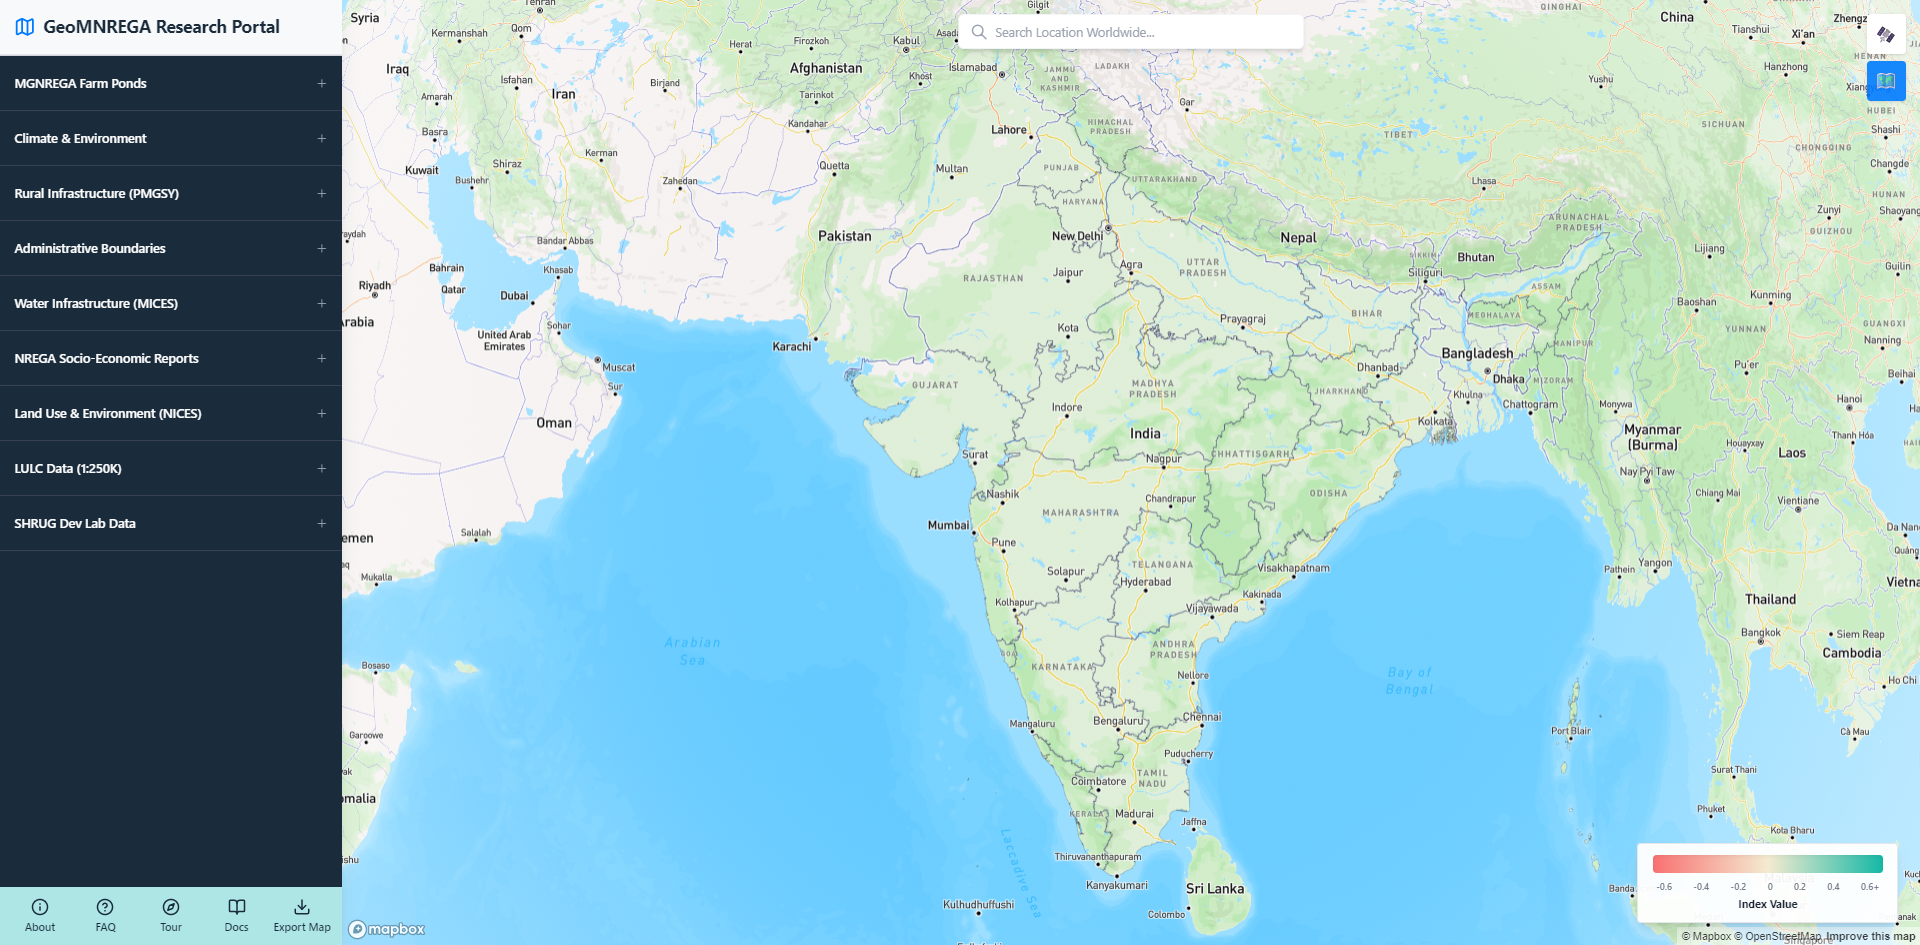
\includegraphics[width=0.9\textwidth]{1.png}
    \caption{Primary Dashboard: National View with Active NREGA Layers}
\end{figure}

\begin{figure}[H]
    \centering
    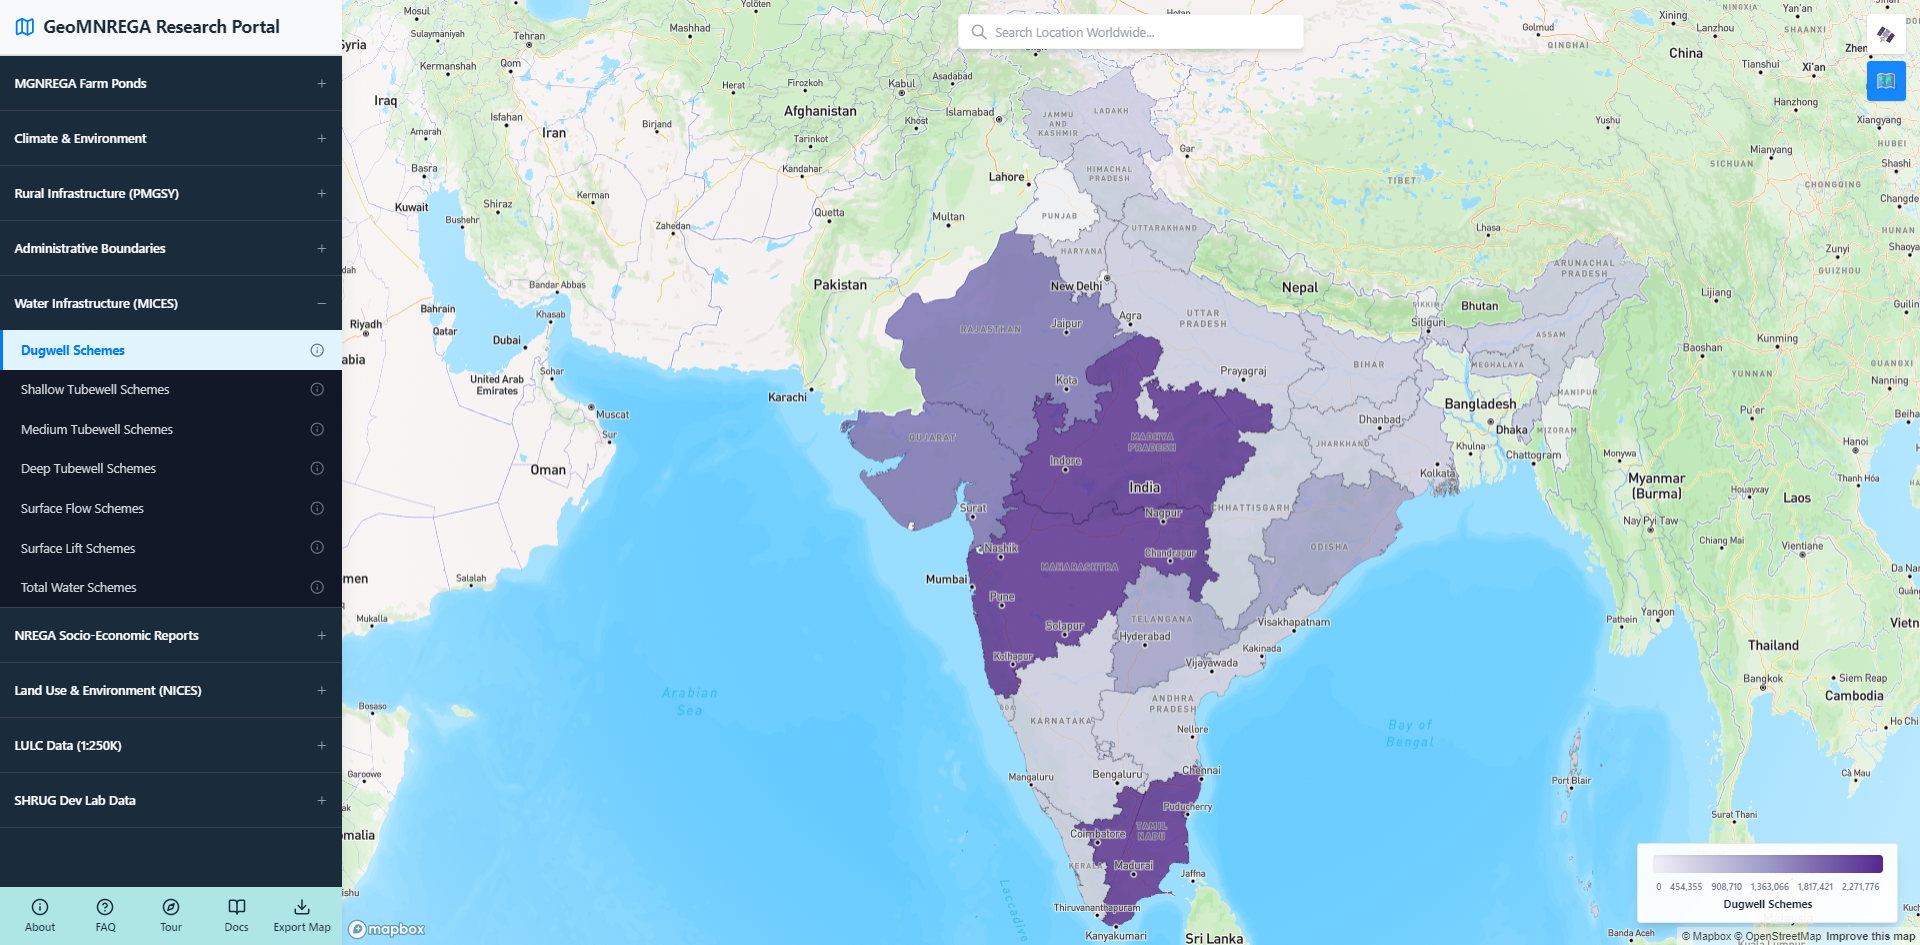
\includegraphics[width=0.9\textwidth]{2.png}
    \caption{Interactive Selection: Sidebar Accordion and Dataset Categories}
\end{figure}

\begin{figure}[H]
    \centering
    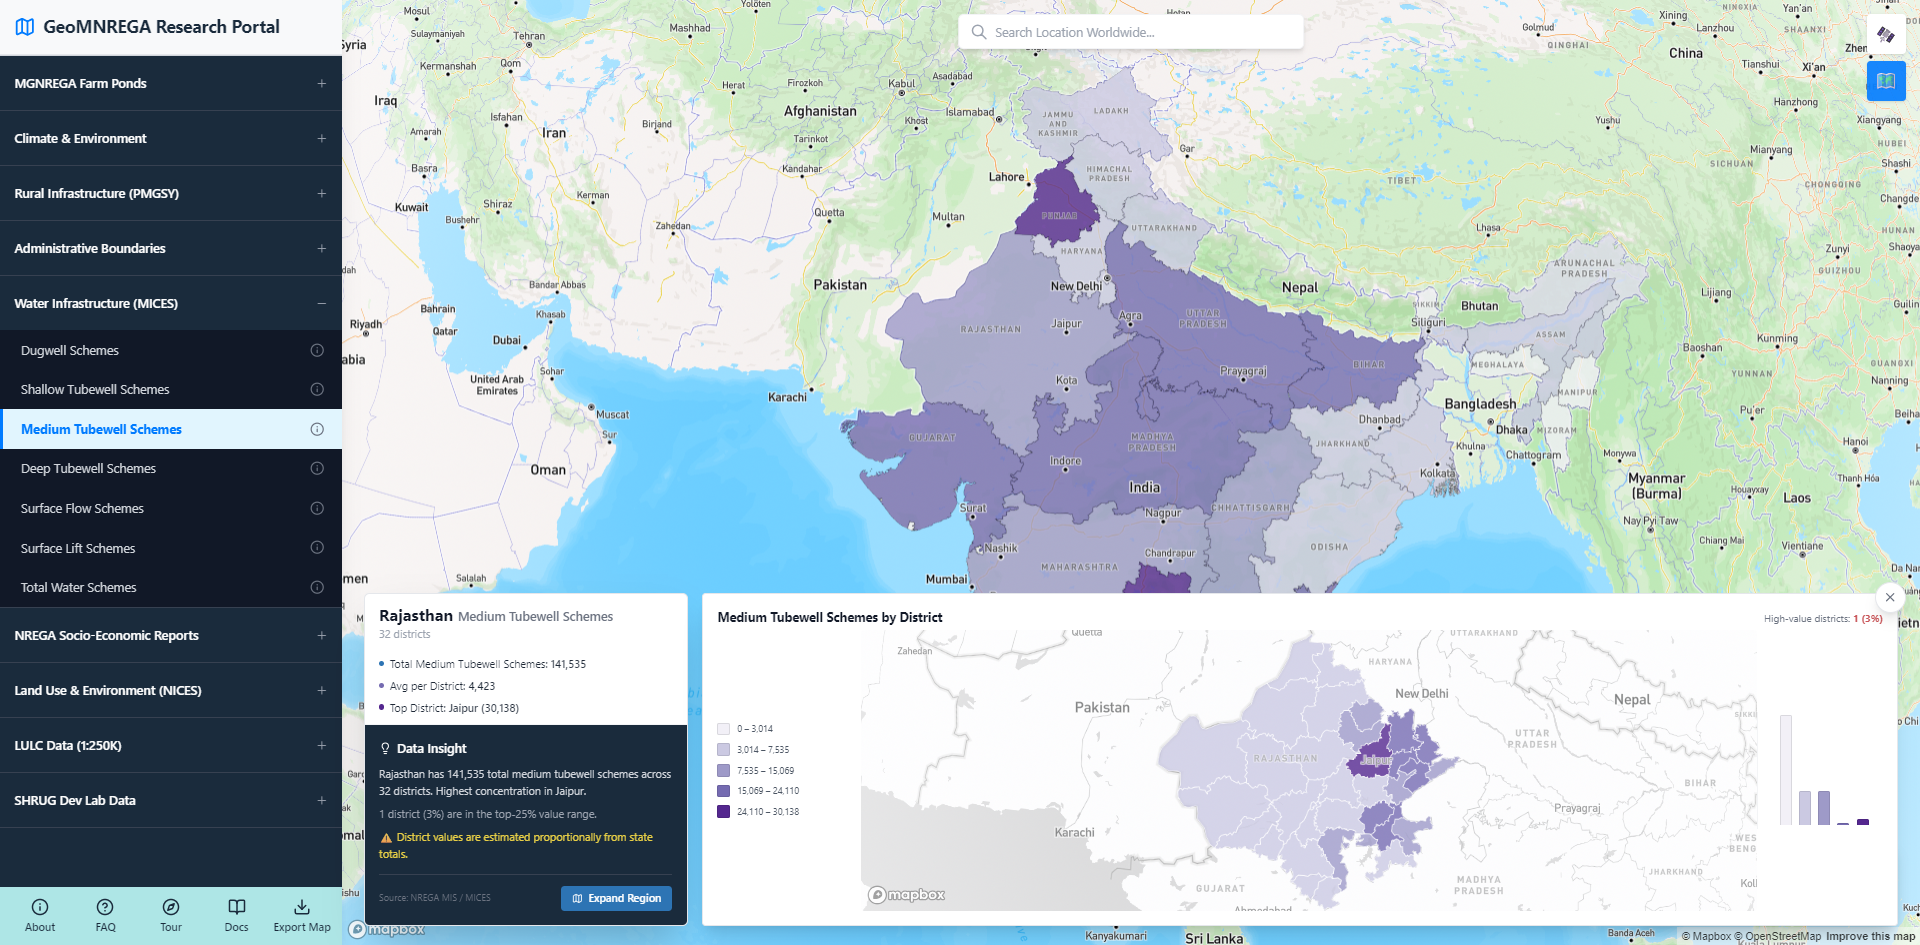
\includegraphics[width=0.9\textwidth]{3.png}
    \caption{State-Level Interaction: Hover Effects and Interactive Map Features}
\end{figure}

\begin{figure}[H]
    \centering
    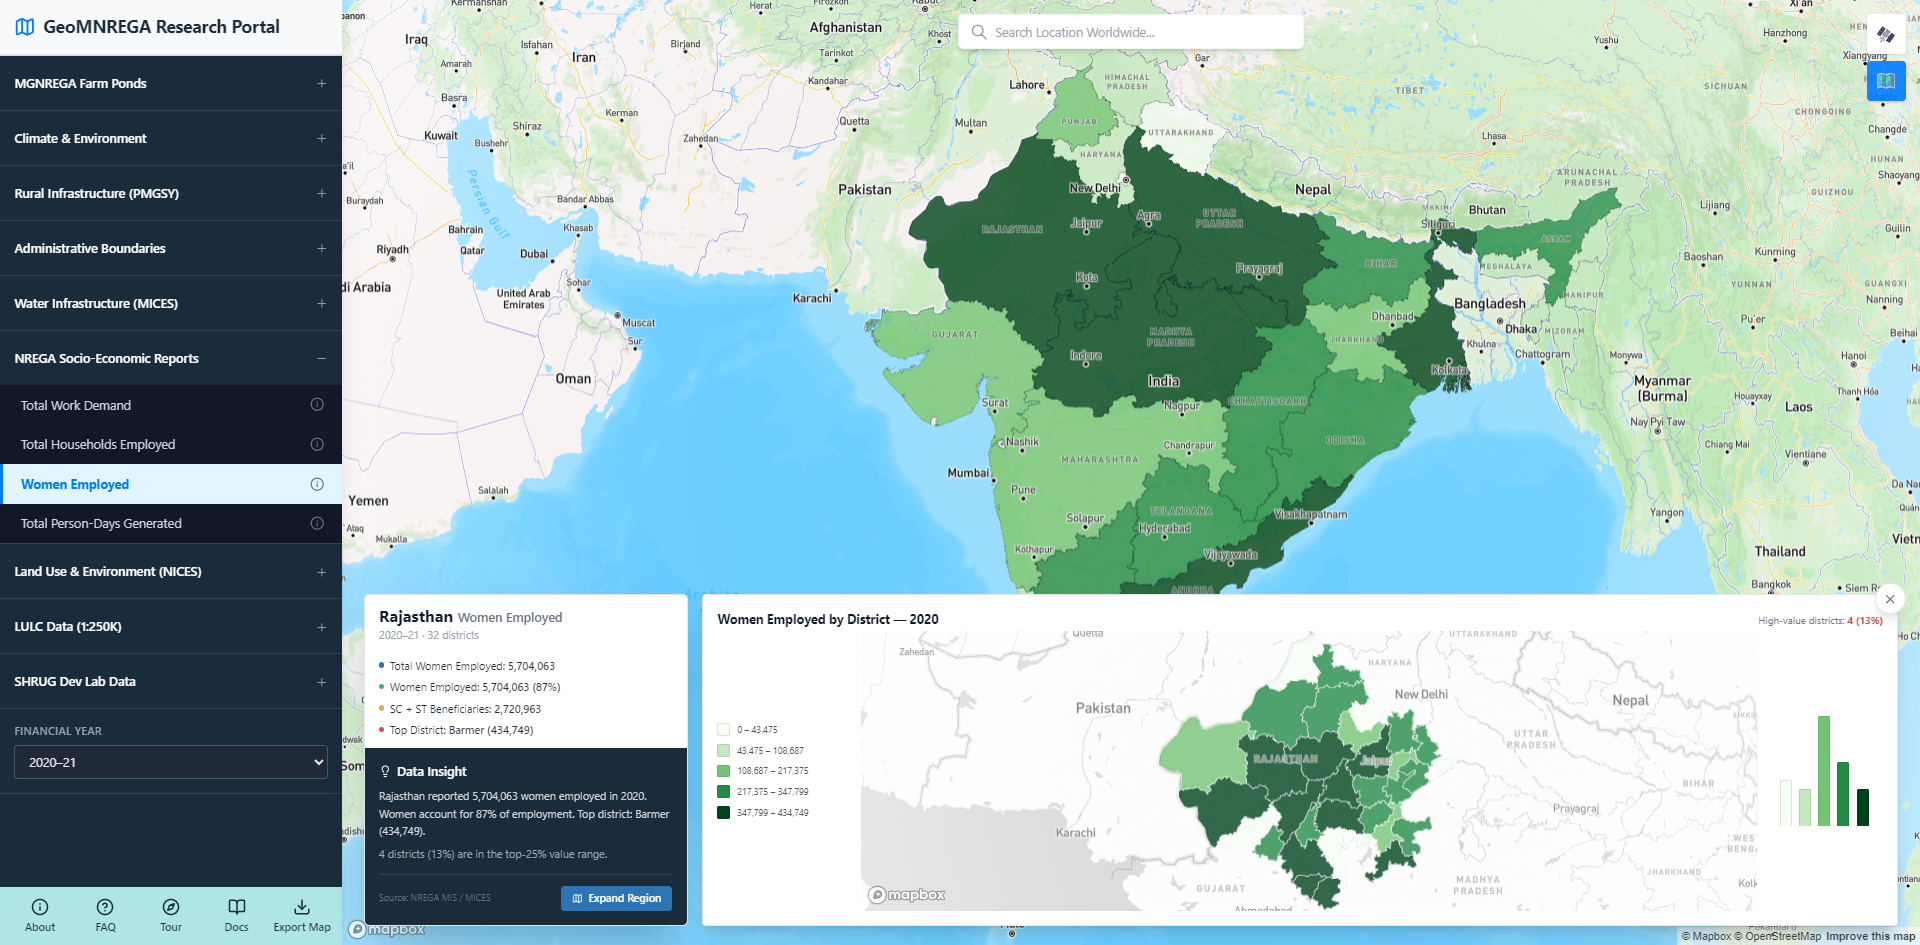
\includegraphics[width=0.9\textwidth]{4.png}
    \caption{Bottom Overlay: Key Performance Indicators for Selected States}
\end{figure}

\begin{figure}[H]
    \centering
    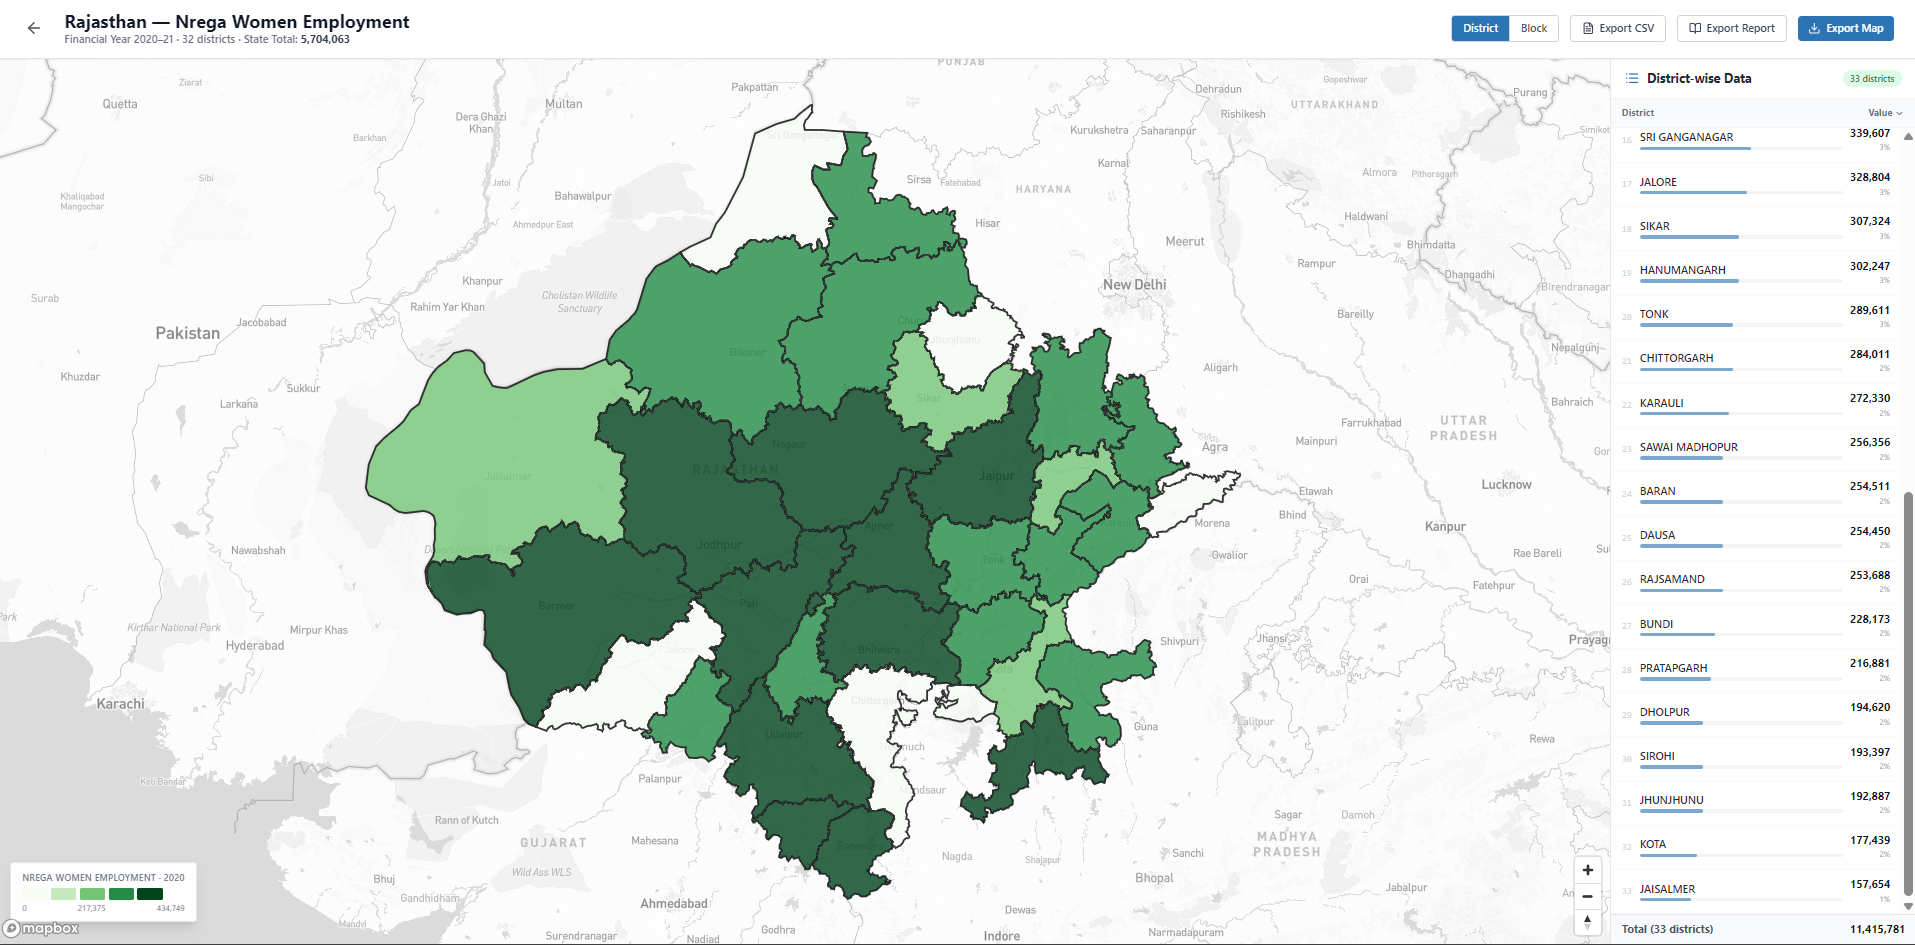
\includegraphics[width=0.9\textwidth]{5.png}
    \caption{Full Drill-Down: State-Specific Research Page with District Rankings}
\end{figure}

\begin{figure}[H]
    \centering
    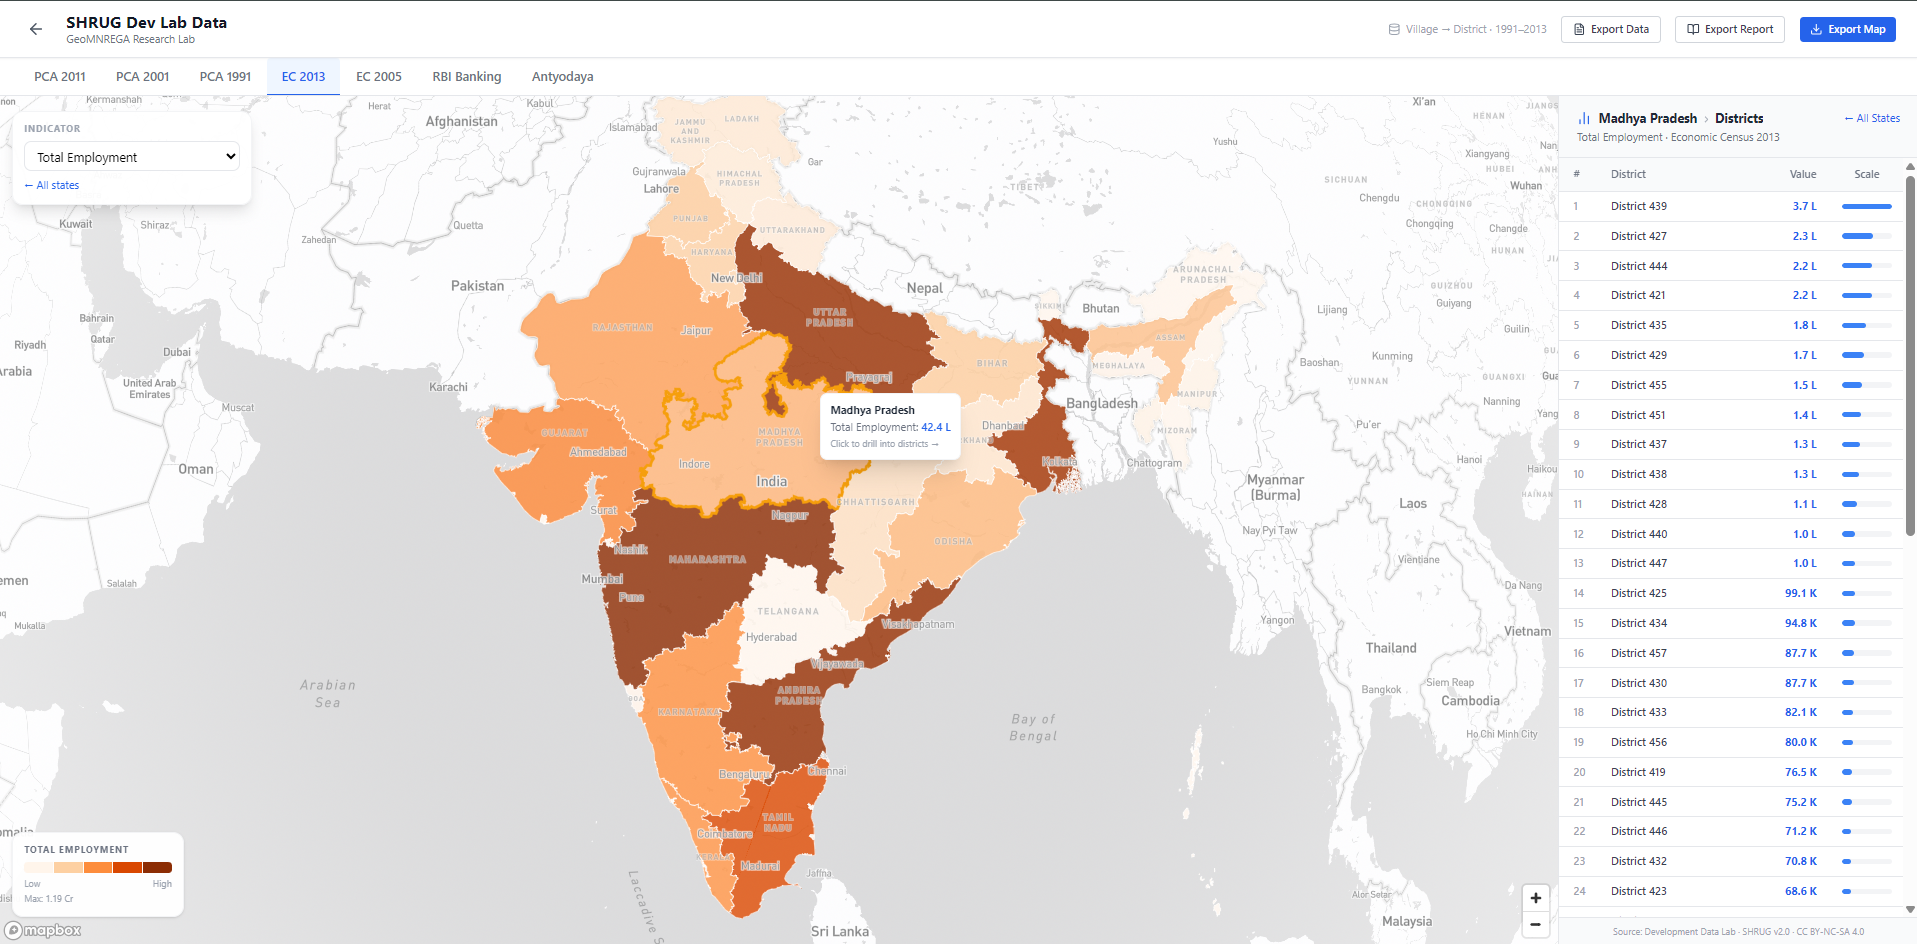
\includegraphics[width=0.9\textwidth]{6.png}
    \caption{District Visualization: MiniMap Component with Sub-State Granularity}
\end{figure}

\begin{figure}[H]
    \centering
    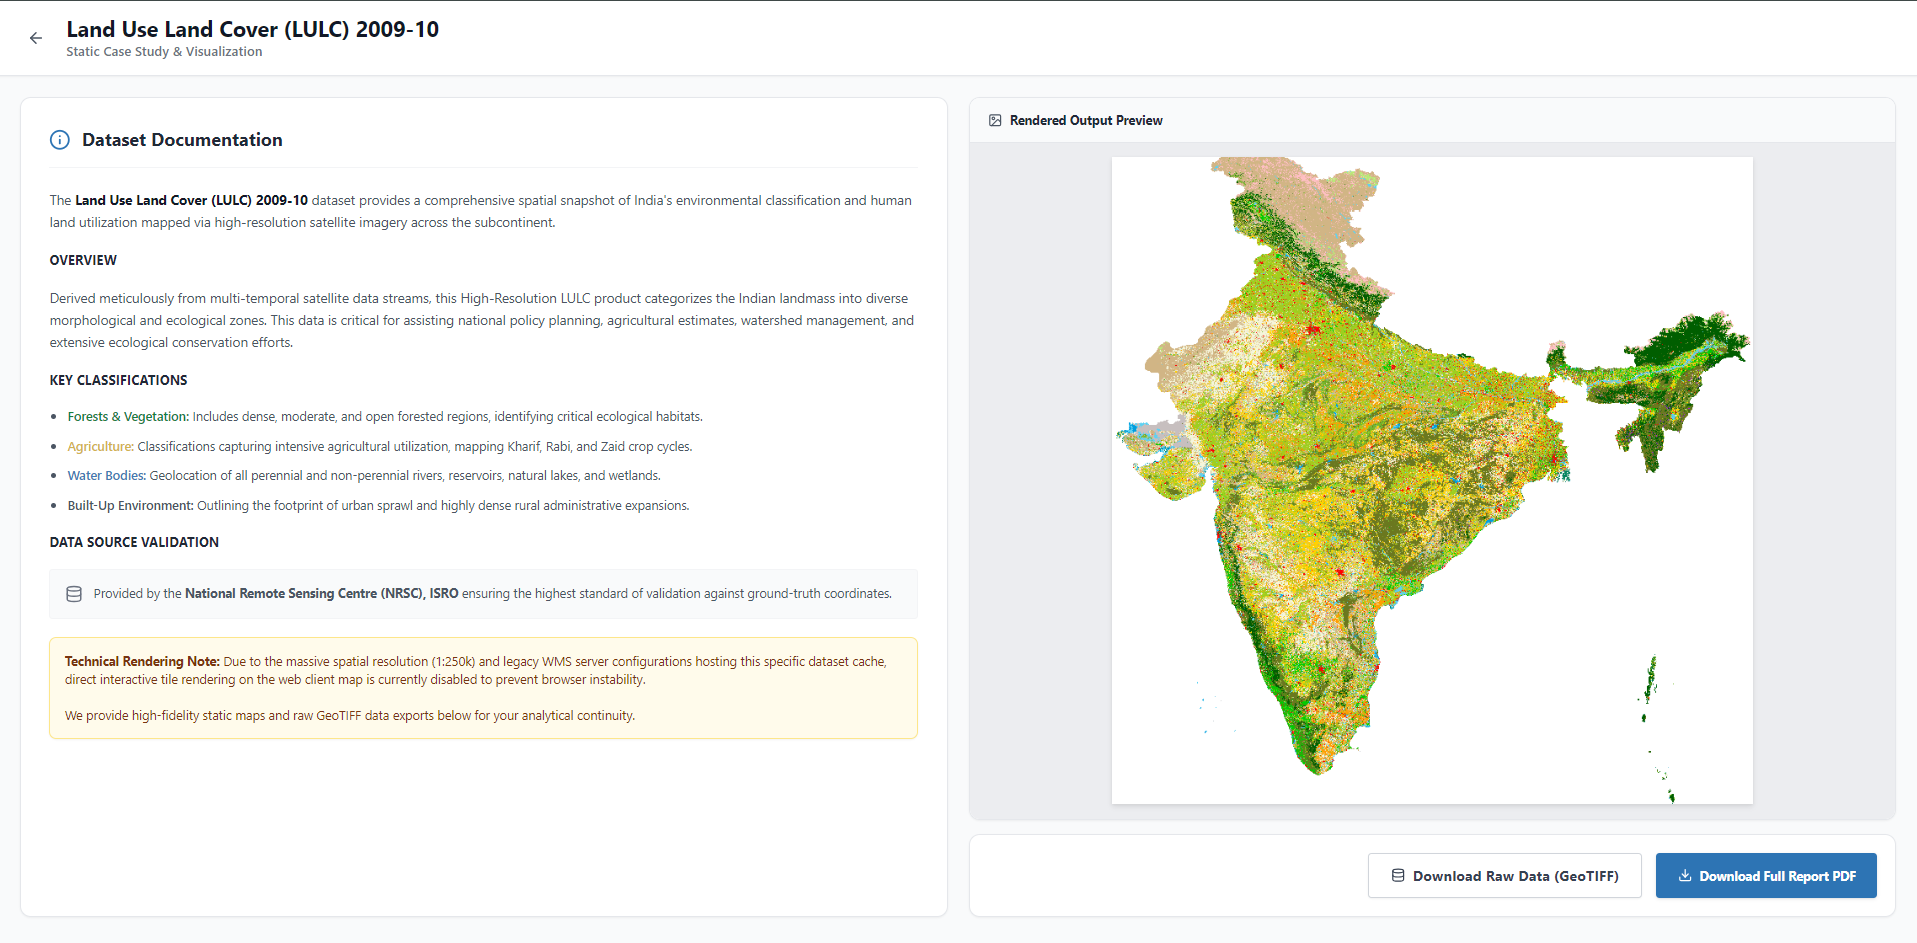
\includegraphics[width=0.9\textwidth]{7.png}
    \caption{LULC Use Case Viewer: Spatial Analysis of Land Use Patterns}
    \label{fig:lulc_viewer}
\end{figure}

\begin{figure}[H]
    \centering
    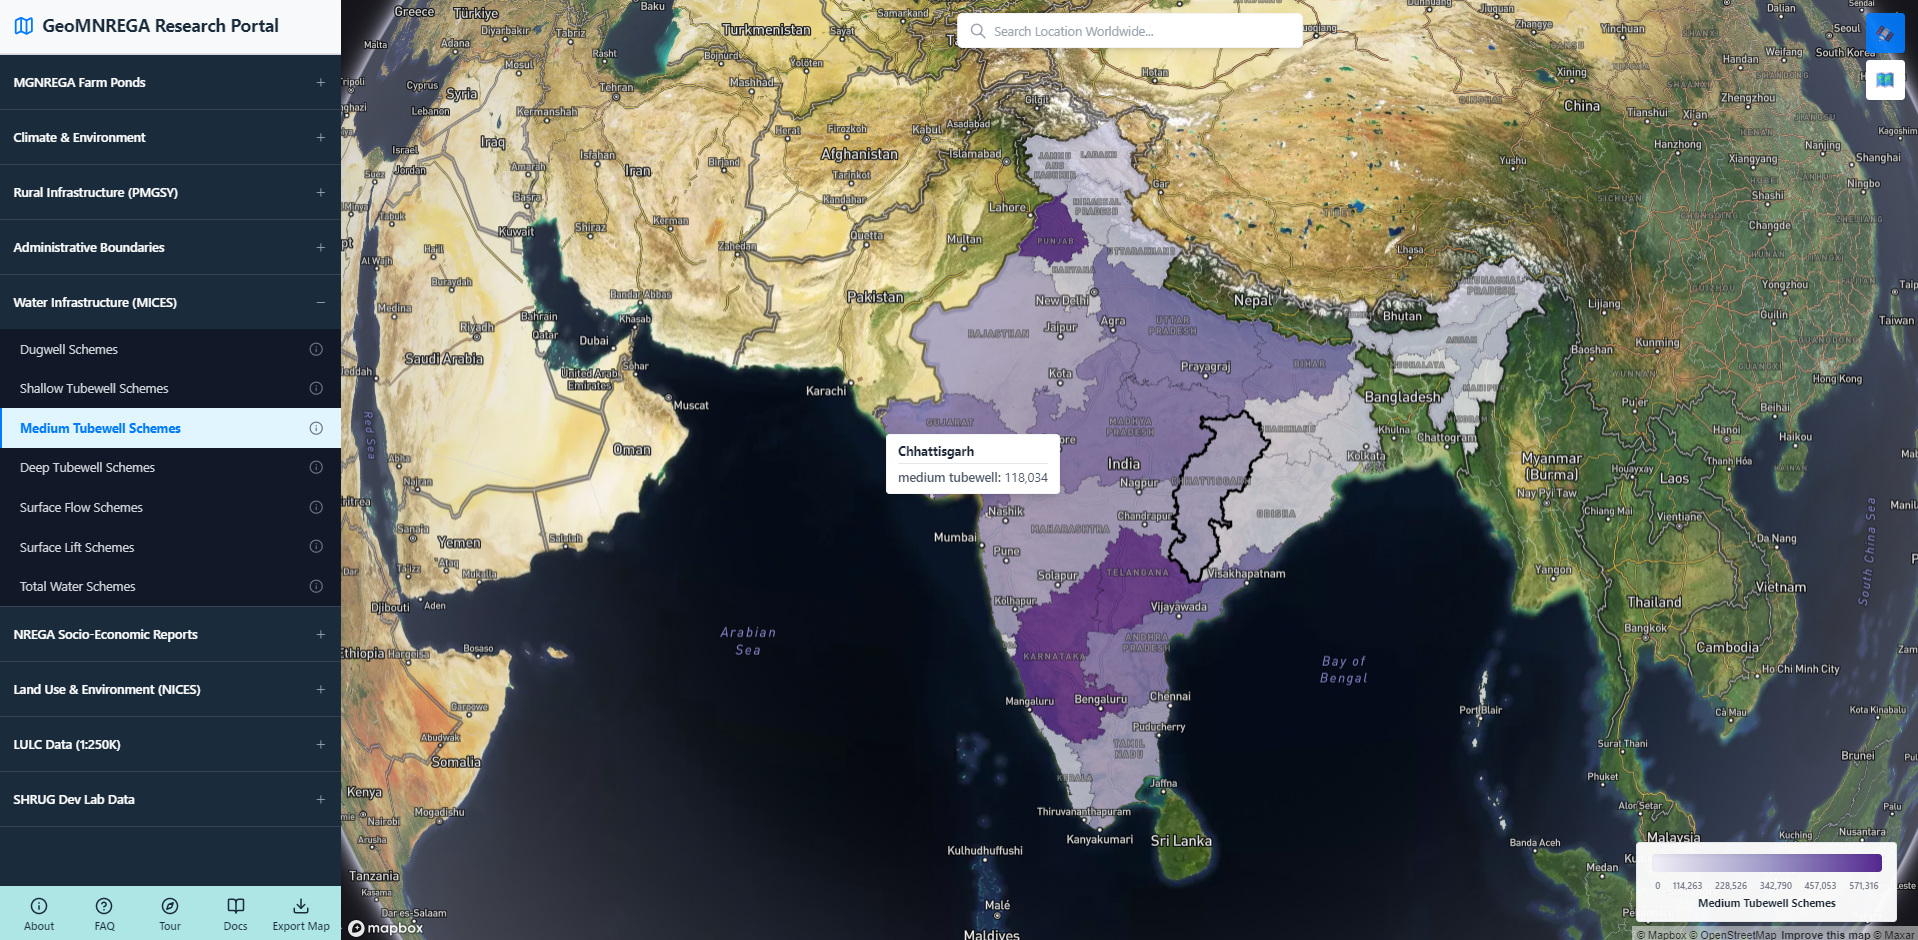
\includegraphics[width=0.9\textwidth]{8.png}
    \caption{Temporal Analysis: Year Selector and Dynamic Data Binding}
\end{figure}

\section{Data Export and Reporting Interface}
The portal provides a professional reporting interface where users can export their spatial findings into a research-ready document format.

\begin{figure}[H]
    \centering
    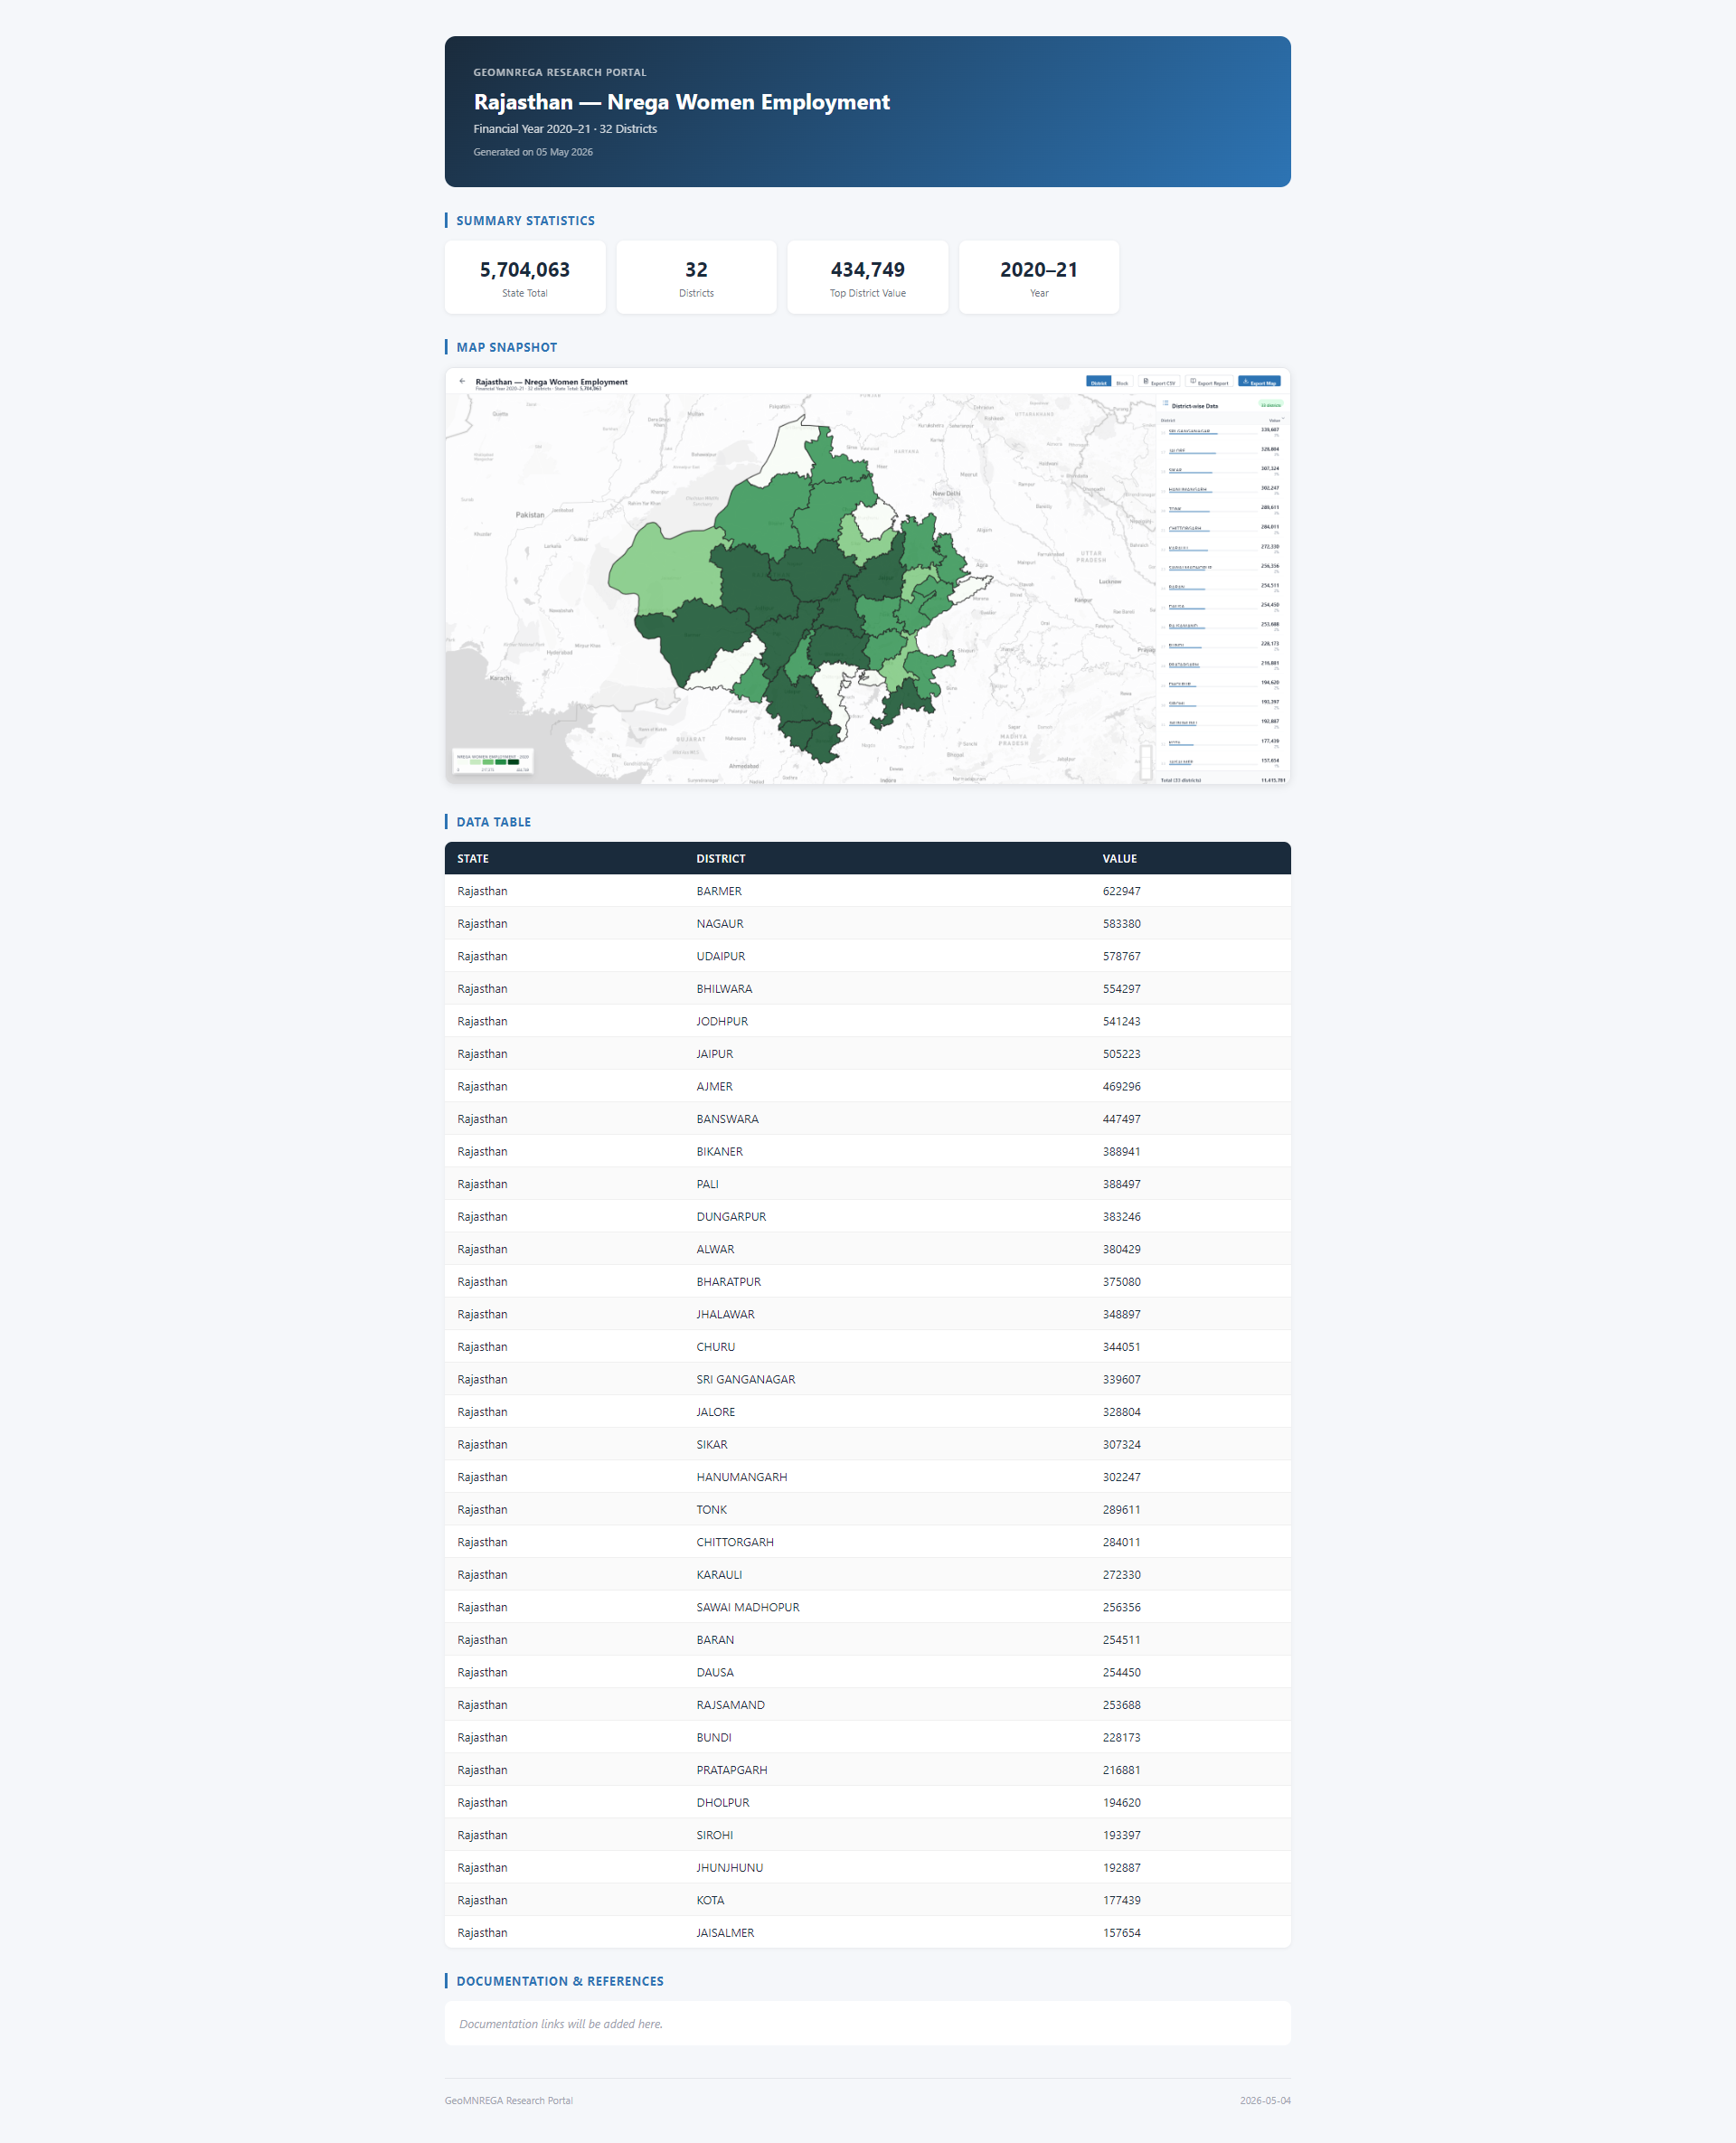
\includegraphics[width=0.8\textwidth]{9.png}
    \caption{Generated Technical Report: Automated PDF Export Preview}
    \label{fig:report_export}
\end{figure}

The generated report includes the active map view, aggregated statistics, and district-wise rankings, formatted for academic and policy-level submission.

\section{Detailed Component Logic: Sidebar}
The \texttt{Sidebar} component is the most complex UI element. It manages a multi-level accordion state.
\begin{lstlisting}[language=javascript, caption={Sidebar Accordion Logic}]
const [openSection, setOpenSection] = useState('nrega');

const toggleSection = (sectionId) => {
  setOpenSection(openSection === sectionId ? null : sectionId);
};
\end{lstlisting}
Each dataset item in the sidebar is rendered dynamically based on a configuration object, ensuring that adding new datasets is as simple as updating a JSON array.

\chapter{Implementation Depth: Critical Functions}

\section{Dynamic Data Injection}
The heart of the visualization is how the frontend maps a selected dataset ID to a GeoJSON property.
\begin{lstlisting}[language=javascript, caption={Dynamic Key Generation}]
const getDataKey = (datasetId, year) => {
  if (datasetId.startsWith('mices_')) {
    return datasetId; // MICES is static
  }
  return `${datasetId}_${year}`; // NREGA is year-specific
};
\end{lstlisting}

\section{State Drill-Down Mechanism}
The transition from a national view to a state view involves coordinate recalculations and bounds fitting.
\begin{lstlisting}[language=javascript, caption={Map Fly-To Logic}]
const handleStateClick = (feature) => {
  const bounds = new mapboxgl.LngLatBounds();
  // Compute bounds from feature geometry
  map.current.flyTo({
    center: feature.properties.centroid,
    zoom: 7,
    essential: true
  });
};
\end{lstlisting}

\chapter{Research Methodology and Data Analysis}

\section{Research Methodology}
The project follows a Quantitative Geospatial Research framework:
\begin{enumerate}
    \item \textbf{Data Acquisition}: Extracting raw reports from official MNREGA and MICES portals.
    \item \textbf{Normalization}: Standardizing state and district names across different datasets (e.g., handling "Odisha" vs "Orissa").
    \item \textbf{Spatial Integration}: Joining tabular data with administrative shapefiles.
    \item \textbf{Visualization Design}: Selecting appropriate color ramps (sequential vs. diverging) for different metric types.
\end{enumerate}

\section{Data Trends Observation}
Based on the visualized datasets, several trends can be analyzed:
\begin{itemize}
    \item \textbf{Employment Correlation}: A visible correlation between work demand and seasonal rainfall patterns across the Central Indian belt.
    \item \textbf{Water Infrastructure Density}: High density of shallow tubewell schemes in the Indo-Gangetic plains compared to dugwells in the Deccan plateau.
    \item \textbf{Women Participation}: Significant growth in women's participation rates in Southern states over the 2018-2022 period.
\end{itemize}

\chapter{User Experience and Design Philosophy}

\section{Design Aesthetic}
The portal adopts a "Premium Research" aesthetic. 
\begin{itemize}
    \item \textbf{Color Palette}: Deep navy (\#1E3A8A) for headers and primary controls, providing a sense of authority.
    \item \textbf{Typography}: Inter and Roboto fonts for high readability of numerical data.
    \item \textbf{Glassmorphism}: Panels use subtle backdrop blurs and semi-transparent backgrounds to maintain spatial context of the underlying map.
\end{itemize}

\section{Responsive Design}
The dashboard is designed for desktop researchers but remains fully functional on tablets. The sidebar collapses into a hamburger menu on smaller screens, and the state dashboard transitions from a side panel to a bottom sheet.

\chapter{Technical Challenges and Solutions}

\section{Handling Geographic Discrepancies}
Administrative boundaries in India are dynamic (e.g., creation of new districts). 
\textbf{Solution:} The project uses a "fuzzy-match" name resolver in the Python preprocessing script to ensure data from 2014-era reports correctly maps to 2024-era GeoJSON geometries.

\section{WebGL Context Limits}
Running multiple map instances (Main Map + MiniMap + State Report Map) can exceed browser WebGL context limits.
\textbf{Solution:} Implementing a singleton pattern for the Mapbox instance or carefully destroying instances on component unmount to free up memory.

\section{Use Case Report (LULC)}
For raster datasets like Land Use Land Cover, Mapbox requires tile servers. To demonstrate this capability in a static environment, clicking an LULC dataset opens the \texttt{UseCaseReport.jsx} overlay. Currently, this acts as a pan-and-zoom image viewer displaying static analytical images.

% ---------------------------------------------------------
% CHAPTER 7: KNOWN GAPS AND FUTURE SCOPE
% ---------------------------------------------------------
\chapter{Testing and Quality Assurance}

\section{Unit Testing}
The project utilizes \texttt{Vitest} for unit testing core logic, such as data key generation and coordinate normalization.
\begin{lstlisting}[language=javascript, caption={Sample Unit Test for Data Key Generator}]
import { describe, it, expect } from 'vitest';
import { getDataKey } from '../utils/mapHelpers';

describe('getDataKey', () => {
  it('returns base key for MICES', () => {
    expect(getDataKey('mices_dugwell', '2020')).toBe('mices_dugwell');
  });
  it('returns year-suffixed key for NREGA', () => {
    expect(getDataKey('nrega_demand', '2021')).toBe('nrega_demand_2021');
  });
});
\end{lstlisting}

\section{Integration Testing}
End-to-end (E2E) tests are implemented using \texttt{Playwright} to ensure that clicking on the map correctly surfaces the dashboard and that sidebar filters update the map's visual state.

\section{Manual Verification}
Given the visual nature of the project, manual cross-referencing with official government portals (e.g., the MNREGA Public Data Portal) is conducted to ensure the accuracy of the displayed choropleth intensities.

\chapter{User Manual: Operating the Portal}

\section{Navigating the Map}
Users can pan the map by clicking and dragging, and zoom using the mouse wheel or the controls in the top-right corner. The search bar at the top allows for quick navigation to specific Indian cities or regions.

\section{Selecting Datasets}
1. Open the \textbf{Sidebar} by clicking the icon on the left.
2. Select a category (e.g., \textit{NREGA Socio-Economic Reports}).
3. Click a dataset (e.g., \textit{Total Households Employed}).
4. The map will update its colors based on the data.

\section{Analyzing Specific Regions}
To view detailed stats for a state, simply click on its polygon. A dashboard will appear at the bottom. To zoom into that state and see district-level data, click the "Expand Region" button within the dashboard.

\chapter{Deployment and Environment Configuration}

\section{Production Build}
The application is optimized for production using Vite's build command:
\begin{lstlisting}[language=bash]
npm run build
\end{lstlisting}
This generates a \texttt{dist/} folder containing minified assets, ready for deployment to platforms like Vercel, Netlify, or AWS S3.

\section{Environment Variables}
A \texttt{.env} file is required at the root of the project to store the Mapbox Access Token:
\begin{lstlisting}[language=text]
VITE_MAPBOX_TOKEN=your_mapbox_public_token_here
\end{lstlisting}

\appendix
\chapter{Code Listing: Python Preprocessing Script}
\begin{lstlisting}[language=python, caption={process\_all\_nrega.py Snippet}]
import json
import pandas as pd

def process_state_data(geojson_path, csv_path, output_path):
    with open(geojson_path, 'r') as f:
        data = json.load(f)
    
    df = pd.read_csv(csv_path)
    
    for feature in data['features']:
        state_name = feature['properties']['NAME_1']
        state_stats = df[df['state'] == state_name]
        
        for _, row in state_stats.iterrows():
            year = row['financial_year']
            feature['properties'][f'nrega_demand_{year}'] = row['demand']
            
    with open(output_path, 'w') as f:
        json.dump(data, f)
\end{lstlisting}

\chapter{Glossary of Terms}
\begin{description}
    \item[MNREGA] Mahatma Gandhi National Rural Employment Guarantee Act.
    \item[MICES] Minor Irrigation Census (Water Infrastructure Data).
    \item[LULC] Land Use Land Cover.
    \item[Choropleth] A thematic map in which areas are shaded or patterned in proportion to a statistical variable.
    \item[GeoJSON] A format for encoding a variety of geographic data structures.
\end{description}

\chapter{Known Gaps and Future Scope}

While the current iteration of the GeoMNREGA Portal is highly functional, several architectural and feature-based enhancements remain.

\section{Current Limitations}
\begin{enumerate}
    \item \textbf{Data Binding in Reports:} In \texttt{StateReport.jsx}, the calculation for the top 10 districts currently utilizes the base property key rather than the year-specific key. This means rankings do not dynamically update when changing the financial year.
    \item \textbf{Unused Components:} Components such as \texttt{Navbar.jsx}, \texttt{Footer.jsx}, and \texttt{ControlPanel.jsx} are present in the repository but remain unrendered.
    \item \textbf{Static LULC Viewer:} The \texttt{UseCaseReport} displays a hardcoded placeholder image regardless of which LULC year is selected.
    \item \textbf{Backend Tile Server:} Rendering NICES raster data (e.g., Cropland maps) currently requires a local tile server running on \texttt{localhost:8000}, limiting production deployment.
\end{enumerate}

\item \textbf{Export Functionality:} Activating the placeholder buttons for exporting data as CSV and reports as PDF documents.
\end{itemize}

\chapter{Frontend Orchestration and Component Logic}
This chapter provides a deep dive into the technical implementation of the user interface, detailing how \textbf{Deepak Meena} orchestrated multiple React components to handle large-scale spatial data interaction without page reloads.

\section{The Sidebar Configuration System}
To ensure the portal is easily extensible, the sidebar does not hardcode its menu items. Instead, it utilizes a \textbf{Dataset Schema} defined in an array of objects. This allows a developer to add a new national-level dataset simply by adding a new entry to the configuration.

\begin{lstlisting}[language=javascript, caption={Sidebar Dataset Configuration Schema}]
const DATASET_CONFIG = [
  {
    id: 'nrega_demand',
    label: 'NREGA Work Demand',
    category: 'Socio-Economic',
    unit: 'Persons',
    scale: 'Sequential'
  },
  {
    id: 'mices_dugwell',
    label: 'MICES Dugwell Count',
    category: 'Water Infrastructure',
    unit: 'Count',
    scale: 'Quantile'
  }
];
\end{lstlisting}

\section{State Management and Prop Drilling}
The application avoids complex global state libraries like Redux to maintain performance. Instead, it utilizes \textbf{React State Lifting}. The \texttt{App.jsx} component holds the "Source of Truth" for:
\begin{enumerate}
    \item \textbf{activeDatasetId}: Which metric is currently being painted on the map.
    \item \textbf{activeYear}: The financial year suffix for the data key.
    \item \textbf{selectedFeature}: The properties of the state/district currently clicked by the user.
\end{enumerate}

\section{Optimized Rendering in StateReport.jsx}
The \texttt{StateReport.jsx} component is responsible for calculating rankings on-the-fly. When a user clicks a state like "Bihar", the component filters the global GeoJSON to extract only Bihar's districts and performs a JavaScript \texttt{sort()} to identify the top-performing areas.

\begin{lstlisting}[language=javascript, caption={On-the-fly District Ranking Logic}]
const getTopDistricts = (allDistricts, stateName, dataKey) => {
  return allDistricts
    .filter(d => d.properties.NAME_1 === stateName)
    .sort((a, b) => b.properties[dataKey] - a.properties[dataKey])
    .slice(0, 10);
};
\end{lstlisting}
This client-side computation ensures that the dashboard feels instantaneous, as no API calls are needed once the GeoJSON is loaded.

\section{Visual Polish: Glassmorphism and Tailwind}
The UI design follows a modern \textbf{Glassmorphism} aesthetic. This is achieved using Tailwind CSS backdrop utilities:
\begin{itemize}
    \item \texttt{bg-white/80}: Provides a semi-transparent white background.
    \item \texttt{backdrop-blur-md}: Creates a frosted glass effect over the underlying Mapbox layer.
    \item \texttt{rounded-xl}: Ensures soft, modern UI corners.
\end{itemize}
This visual style ensures that the map remains visible even when reports are open, providing continuous spatial context to the researcher.

\section{Proposed Project: Population Raster Map for India}
Based on the foundational work of the GeoMNREGA portal and under the guidance of \textbf{Gaurav Arora}, a significant research extension is proposed: the development of a high-resolution, India-specific population raster map.

\subsection{Objective and Motivation}
We propose to initiate the development of a high-resolution population raster map for India as a foundational step towards building a comprehensive geospatial data platform. In the first phase, the objective is to construct a preliminary population surface using \textbf{Census 2011} village and town-level population data, combined with spatial boundary datasets such as \textbf{GramChitra} (village/GP boundaries) and administrative layers. 

Since individual-level geolocation data (exact addresses or person-level coordinates) is not publicly available due to privacy constraints, the approach relies on spatially distributing aggregated population data within known geographic boundaries.

\subsection{Methodology: Dasymetric Mapping using LULC}
The initial version will follow a simple uniform distribution approach, where population is evenly spread across each village polygon. However, this assumption is unrealistic because population is not uniformly distributed—people live in settlements, not forests or water bodies. 

To address this, the project will incorporate \textbf{Land Use Land Cover (LULC)} data as an auxiliary dataset to refine the distribution. It is important to clarify the distinction between these datasets:
\begin{itemize}
    \item \textbf{LULC Raster:} A categorical dataset that classifies land into types such as built-up areas, cropland, forest, and water (i.e., what exists on the land).
    \item \textbf{Population Raster:} A quantitative dataset representing \textit{how many people live} in each specific location.
\end{itemize}
In this project, LULC will be used as a guiding layer to ensure that population is allocated primarily to habitable zones (built-up areas) rather than being spread uniformly across all land types. This technique, known as \textbf{Dasymetric Mapping}, has been used for global-scale maps, but our proposal focuses on creating an \textbf{India-specific map} derived from high-resolution localized datasets like the 2011 Census and GramChitra.

\subsection{Technical Specifications and Future Scope}
The refined population distribution will be converted into a raster grid at a chosen resolution:
\begin{itemize}
    \item \textbf{High Precision:} 5 km $\times$ 5 km.
    \item \textbf{Optimal Balance:} 10 km $\times$ 10 km (Recommended).
\end{itemize}
Each pixel in this grid will represent the estimated population count within that spatial unit. This raster format allows for continuous spatial analysis and seamless integration with other datasets such as climate, infrastructure, and environmental layers.

The resulting population raster will serve as a \textbf{proof-of-concept dataset}, which can later be improved using updated census data, additional proxies (e.g., night-time lights, infrastructure density), and more advanced modeling techniques. Applications include urban planning, infrastructure allocation, disaster response planning, and spatial-economic analysis.

% ---------------------------------------------------------
% CHAPTER 8: CONCLUSION
% ---------------------------------------------------------
\chapter{Conclusion}
The GeoMNREGA Portal successfully demonstrates how modern web technologies can be orchestrated to build a highly interactive, performant, and visually appealing spatial research dashboard. By meticulously preprocessing raw government data into GeoJSON and rendering it via WebGL in the browser, the application empowers researchers to derive geographic insights instantaneously. Addressing the known gaps and migrating to a dynamic backend will solidify this project as a robust tool for public policy analysis.

\end{spacing}
\end{document}
